\documentclass[aspectratio=169]{beamer}

\usepackage[utf8]{inputenc}
\usepackage[T1]{fontenc}
\usepackage{amsmath,amssymb,amsfonts,bm,mathtools}
\usepackage{physics}
\usepackage{braket}
\usepackage{hyperref}
\usepackage{tikz}
\usetikzlibrary{positioning,arrows.meta}

\usetheme{Madrid}

\title{Agentic AI, Reinforcement Learning, and Quantum Control}
\subtitle{Toward Hybrid RL + Agentic Systems for Physics Problems}
\author{Morten Hjorth-Jensen}
\date{April 23, 2026}

\begin{document}

\frame{\titlepage}

\begin{frame}{Aim of These Notes}
These slides develop three related ideas:
\begin{enumerate}
    \item the conceptual link between reinforcement learning (RL) and agentic AI,
    \item how this link appears naturally in quantum control,
    \item how to build a hybrid RL + agentic system for physics problems.
\end{enumerate}

\medskip

The guiding perspective is that quantum control is inherently a sequential decision-making problem, while agentic AI provides a higher-level architecture for planning, tool use, and adaptive workflow management.
\end{frame}

\section{Reinforcement learning and agentic AI}

\begin{frame}{Reinforcement Learning}
In reinforcement learning, an agent interacts with an environment over time:
\[
s_t \rightarrow a_t \rightarrow r_t, s_{t+1}.
\]

The objective is to maximize expected cumulative reward,
\[
J(\pi)=\mathbb{E}_\pi\left[\sum_{t=0}^{T-1}\gamma^t r_t\right],
\]
where:
\begin{itemize}
    \item \(s_t\) is the state,
    \item \(a_t\) is the action,
    \item \(r_t\) is the reward,
    \item \(\pi(a|s)\) is the policy.
\end{itemize}
\end{frame}

\begin{frame}{Agentic AI}
Agentic AI refers to systems that:
\begin{itemize}
    \item pursue explicit goals,
    \item make multi-step plans,
    \item use tools,
    \item adapt to feedback,
    \item and coordinate longer workflows.
\end{itemize}

It is broader than RL. A modern agentic system may combine:
\begin{itemize}
    \item planning,
    \item memory,
    \item search,
    \item external simulation tools,
    \item and learned controllers.
\end{itemize}
\end{frame}

\begin{frame}{The Link Between Them}
The connection is:
\[
\boxed{
\text{RL is a mathematical training framework for agents, while agentic AI is a broader system architecture for autonomous goal-directed behavior.}
}
\]

RL gives:
\begin{itemize}
    \item a formal theory of sequential decision-making,
    \item value functions and policies,
    \item rewards and long-horizon optimization.
\end{itemize}

Agentic AI adds:
\begin{itemize}
    \item planning over tasks,
    \item decomposition of objectives,
    \item tool orchestration,
    \item meta-level strategy.
\end{itemize}
\end{frame}

\section{Quantum control as a sequential decision problem}

\begin{frame}{Quantum Control Problem}
A standard controlled Hamiltonian has the form
\[
H(t)=H_d+\sum_{k} u_k(t) H_k,
\]
where:
\begin{itemize}
    \item \(H_d\) is the drift Hamiltonian,
    \item \(H_k\) are control Hamiltonians,
    \item \(u_k(t)\) are external control amplitudes.
\end{itemize}

The goal is to choose \(u_k(t)\) so that the evolution
\[
i\frac{d}{dt}\ket{\psi(t)} = H(t)\ket{\psi(t)}
\]
implements a desired state transfer or target gate.
\end{frame}

\begin{frame}{Control Objective}
For a target unitary \(U_{\mathrm{target}}\), one often maximizes a gate fidelity such as
\[
F = \frac{1}{d^2}\left|\Tr\left(U_{\mathrm{target}}^\dagger U(T)\right)\right|^2.
\]

Equivalently, one minimizes an infidelity
\[
\epsilon = 1-F.
\]

A practical control objective may also include penalties:
\[
\mathcal{J}[u]
=
1-F
+ \lambda_1 \mathcal{C}_{\mathrm{amp}}
+ \lambda_2 \mathcal{C}_{\mathrm{smooth}}
+ \lambda_3 \mathcal{C}_{\mathrm{leak}}.
\]

This already looks like a reward engineering problem.
\end{frame}

\begin{frame}{Why Quantum Control Looks Like RL}
Discretize time into \(N_t\) steps:
\[
t_0,t_1,\dots,t_{N_t}.
\]

Then:
\begin{itemize}
    \item state \(s_t\): current wavefunction, propagator, or reduced feature representation,
    \item action \(a_t\): control amplitude update \(u_k(t)\),
    \item environment: Schr\"odinger evolution or open-system simulator,
    \item reward \(r_t\): fidelity increment, final fidelity, or penalized objective.
\end{itemize}

So the control problem becomes:
\[
\text{choose actions over time to maximize final quantum performance.}
\]
\end{frame}

\begin{frame}{MDP View of Quantum Control}
The controlled quantum dynamics define a Markov decision process:
\[
\mathcal{M}=(\mathcal{S},\mathcal{A},P,R).
\]

One may choose:
\begin{align*}
\mathcal{S} &: \text{Bloch vectors, amplitudes, density matrix features, fidelities, leakage levels},\\
\mathcal{A} &: \text{pulse amplitudes, phases, frequencies, durations},\\
P &: \text{quantum dynamics + noise model},\\
R &: \text{reward based on gate fidelity, robustness, smoothness, runtime}.
\end{align*}

This is why RL has become natural in quantum control.
\end{frame}

\begin{frame}{Classical Quantum-Control Methods vs RL}
Traditional methods:
\begin{itemize}
    \item GRAPE,
    \item Krotov,
    \item CRAB,
    \item Pontryagin-inspired optimal control.
\end{itemize}

These are powerful when:
\begin{itemize}
    \item gradients are accessible,
    \item the model is known,
    \item the optimization landscape is manageable.
\end{itemize}

RL becomes attractive when:
\begin{itemize}
    \item feedback is delayed,
    \item robustness matters,
    \item noise and uncertainty are significant,
    \item one wants adaptive or closed-loop behavior.
\end{itemize}
\end{frame}

\section{How agentic AI enters quantum control}

\begin{frame}{Why RL Alone Is Not the Whole Story}
RL optimizes a policy inside a fixed environment and reward structure.

But realistic physics problems often require additional tasks:
\begin{itemize}
    \item selecting the control model,
    \item choosing a simulation fidelity,
    \item changing the reward definition,
    \item diagnosing failure modes,
    \item comparing methods,
    \item adapting to experimental data.
\end{itemize}

These are naturally agentic tasks.
\end{frame}

\begin{frame}{Agentic Layer Above Quantum Control}
A higher-level agent can:
\begin{itemize}
    \item choose whether to use GRAPE, RL, Bayesian optimization, or hybrid methods,
    \item call simulation tools,
    \item inspect fidelities, leakage, and robustness,
    \item refine pulse parametrizations,
    \item trigger retraining under new constraints,
    \item summarize and compare candidate controllers.
\end{itemize}

So RL can be one module inside a broader agentic architecture.
\end{frame}

\begin{frame}{Two-Level Architecture}
A useful conceptual split is:

\medskip

\textbf{Low level:}
\begin{itemize}
    \item a learned controller or RL policy that outputs pulse actions.
\end{itemize}

\textbf{High level:}
\begin{itemize}
    \item an agentic planner that decides which tasks to run, which models to trust, and how to adapt the workflow.
\end{itemize}

In shorthand:
\[
\text{Agentic planner} \longrightarrow \text{RL controller} \longrightarrow \text{quantum system}.
\]
\end{frame}

\section{Hybrid RL + agentic systems for physics}

\begin{frame}{General Hybrid RL + Agentic System}
A generic architecture for physics problems contains:
\begin{enumerate}
    \item a \textbf{planner},
    \item one or more \textbf{physics simulators},
    \item an \textbf{RL controller},
    \item an \textbf{evaluator},
    \item a \textbf{memory / experiment log},
    \item a \textbf{policy for adaptation}.
\end{enumerate}

This is useful whenever the problem is too complicated to solve with a single optimizer alone.
\end{frame}

\begin{frame}{Architecture Diagram}
\centering
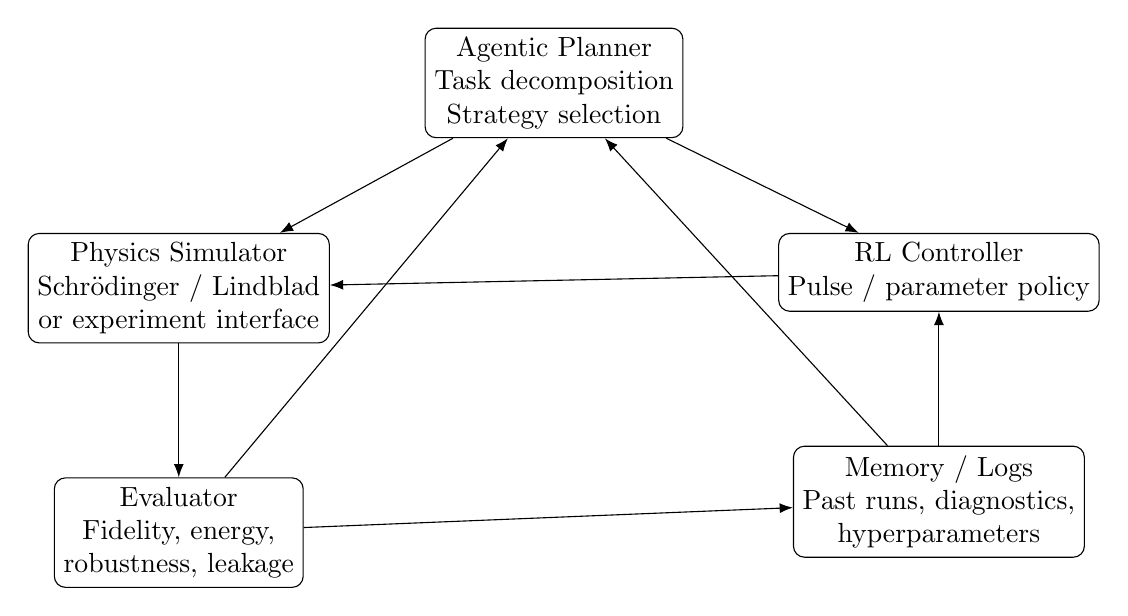
\begin{tikzpicture}[node distance=1.7cm, >=Latex]
\node[draw, rounded corners, align=center] (planner) {Agentic Planner\\Task decomposition\\Strategy selection};
\node[draw, rounded corners, below left=of planner, align=center] (sim) {Physics Simulator\\Schr\"odinger / Lindblad\\or experiment interface};
\node[draw, rounded corners, below right=of planner, align=center] (rl) {RL Controller\\Pulse / parameter policy};
\node[draw, rounded corners, below=of sim, align=center] (eval) {Evaluator\\Fidelity, energy,\\robustness, leakage};
\node[draw, rounded corners, below=of rl, align=center] (mem) {Memory / Logs\\Past runs, diagnostics,\\hyperparameters};

\draw[->] (planner) -- (sim);
\draw[->] (planner) -- (rl);
\draw[->] (rl) -- (sim);
\draw[->] (sim) -- (eval);
\draw[->] (eval) -- (planner);
\draw[->] (eval) -- (mem);
\draw[->] (mem) -- (planner);
\draw[->] (mem) -- (rl);
\end{tikzpicture}
\end{frame}

\begin{frame}{What the Agentic Planner Actually Does}
The planner can perform tasks like:
\begin{itemize}
    \item define the target task,
    \item choose the state representation,
    \item choose the reward,
    \item choose the controller family,
    \item request more data,
    \item switch between coarse and fine simulations,
    \item compare candidate policies,
    \item terminate or continue search.
\end{itemize}

This is more like scientific workflow management than standard RL.
\end{frame}

\section{Explicit quantum-control example}

\begin{frame}{Example: Two-Qubit Gate Synthesis}
Suppose we want to synthesize a target two-qubit gate \(U_\star\) under the Hamiltonian
\[
H(t)=H_d + u_x^{(1)}(t)X_1 + u_y^{(1)}(t)Y_1 + u_x^{(2)}(t)X_2 + u_y^{(2)}(t)Y_2.
\]

The RL controller chooses the controls
\[
a_t = \big(u_x^{(1)}(t),u_y^{(1)}(t),u_x^{(2)}(t),u_y^{(2)}(t)\big).
\]

The agentic planner decides:
\begin{itemize}
    \item whether to optimize a CZ or iSWAP gate,
    \item whether to include noise,
    \item whether to penalize leakage strongly,
    \item whether to use RL or switch to GRAPE for final polishing.
\end{itemize}
\end{frame}

\begin{frame}{Reward Design in Hybrid Quantum Control}
A typical RL reward might be
\[
r_T = \alpha F_T - \beta L_T - \gamma P_T,
\]
where:
\begin{itemize}
    \item \(F_T\): target fidelity,
    \item \(L_T\): leakage penalty,
    \item \(P_T\): pulse power or roughness penalty.
\end{itemize}

A more shaped reward could be
\[
r_t = \Delta F_t - \lambda_1 \Delta L_t - \lambda_2 \abs{a_t}^2.
\]

The agentic layer can modify the coefficients \(\alpha,\beta,\gamma,\lambda_i\) depending on the current training stage.
\end{frame}

\begin{frame}{Example Agentic Strategy}
A realistic multi-stage strategy:
\begin{enumerate}
    \item use coarse simulation and cheap RL training to find rough pulses,
    \item evaluate robustness to detuning and decoherence,
    \item if good, switch to higher-fidelity simulation,
    \item re-optimize with a refined reward,
    \item optionally hand off to GRAPE for local polishing,
    \item validate on noisy and perturbed models.
\end{enumerate}

This is exactly the type of behavior that a pure RL loop does not naturally organize on its own.
\end{frame}

\section{Beyond quantum control: physics problems more broadly}

\begin{frame}{Hybrid RL + Agentic Systems for Physics Problems}
The same architecture applies beyond quantum control.

Examples:
\begin{itemize}
    \item adaptive experiment design,
    \item quantum sensing,
    \item materials search,
    \item PDE-constrained optimization,
    \item active learning for phase diagrams,
    \item variational many-body wavefunction optimization.
\end{itemize}

The common structure is:
\[
\text{sequential control or design} + \text{simulation / experiment} + \text{higher-level planning}.
\]
\end{frame}

\begin{frame}{Example: Quantum Sensing}
In sensing, the RL controller may optimize:
\begin{itemize}
    \item interrogation times,
    \item control pulses,
    \item measurement bases,
    \item adaptive feedback rules.
\end{itemize}

The agentic layer may:
\begin{itemize}
    \item choose which parameter to estimate first,
    \item switch protocols depending on current uncertainty,
    \item decide when to collect more data,
    \item compare strategies using Fisher information or QFI.
\end{itemize}
\end{frame}

\begin{frame}{Example: Variational Many-Body Physics}
In many-body optimization, an RL component may tune:
\begin{itemize}
    \item variational parameters,
    \item Monte Carlo update proposals,
    \item annealing schedules.
\end{itemize}

The agentic layer may:
\begin{itemize}
    \item choose ansatz families,
    \item switch sampling strategies,
    \item inspect convergence and variance,
    \item refine the search over model classes.
\end{itemize}
\end{frame}

\section{Mathematical viewpoint}

\begin{frame}{Hierarchical Optimization View}
One can formalize the hybrid system as a bilevel optimization problem.

Low level:
\[
\pi_\phi^\star = \arg\max_{\pi_\phi} J(\pi_\phi; c),
\]
where \(c\) denotes context or task settings chosen by the higher-level agent.

High level:
\[
c^\star = \arg\max_c \mathcal{U}\big(\pi_\phi^\star(c), \mathcal{D}, \mathcal{M}\big),
\]
where:
\begin{itemize}
    \item \(\mathcal{D}\) may be data or logs,
    \item \(\mathcal{M}\) may be model choice or simulation settings.
\end{itemize}

So the agentic system optimizes the context in which RL itself is run.
\end{frame}

\begin{frame}{Control, Estimation, and Meta-Decision}
There are really three layers:
\begin{enumerate}
    \item \textbf{dynamics:} Schr\"odinger / Lindblad / PDE evolution,
    \item \textbf{control:} optimize actions for a fixed task,
    \item \textbf{meta-decision:} choose the task framing, tools, and adaptation logic.
\end{enumerate}

RL naturally occupies layer 2.

Agentic AI naturally occupies layer 3.
\end{frame}

\section{Practical implementation sketch}

\begin{frame}{Implementation Sketch}
A concrete implementation might use:
\begin{itemize}
    \item simulator: QuTiP, custom NumPy/SciPy, or experiment API,
    \item RL backend: PPO, TRPO, SAC, or policy-gradient method,
    \item planner: LLM-based or rule-based orchestration layer,
    \item memory: database of runs, fidelities, hyperparameters,
    \item evaluator: scripts for robustness, leakage, spectra, or QFI.
\end{itemize}

The planner does not need to solve the physics itself. It coordinates tools that do.
\end{frame}

\begin{frame}[fragile]{Minimal Pseudocode}
\begin{verbatim}
while budget_not_exhausted:
    task = planner.choose_task(memory)
    env  = build_environment(task)
    policy = train_or_update_rl(env, memory)
    result = evaluate(policy, env)
    memory.store(task, policy, result)
    planner.update(memory)
\end{verbatim}

The key point is that the planner is not merely an optimizer; it is a controller of the overall scientific workflow.
\end{frame}

\section{Advantages and limitations}

\begin{frame}{Why This Hybrid Approach Is Attractive}
Advantages:
\begin{itemize}
    \item combines long-horizon control with scientific workflow reasoning,
    \item handles changing objectives and constraints,
    \item can adapt to uncertainty and noise,
    \item supports tool use and model selection,
    \item is well suited to realistic physics pipelines.
\end{itemize}
\end{frame}

\begin{frame}{Limitations and Cautions}
Challenges:
\begin{itemize}
    \item reward misspecification,
    \item simulation cost,
    \item instability of RL training,
    \item hard credit assignment,
    \item planner errors or overconfident meta-decisions,
    \item difficulty of formal guarantees.
\end{itemize}

So the architecture is powerful, but it must be used carefully and benchmarked against simpler baselines.
\end{frame}

\section{Summary}

\begin{frame}{Take-Home Summary}
The main points are:
\begin{itemize}
    \item RL and agentic AI are linked because both concern sequential goal-directed action.
    \item Quantum control is naturally an RL problem once time is discretized and controls become actions.
    \item Realistic physics workflows often need more than RL alone; they need planning, tool use, and adaptation.
    \item A hybrid RL + agentic system separates:
    \[
    \text{high-level planning} \quad \text{from} \quad \text{low-level control}.
    \]
\end{itemize}
\end{frame}

\begin{frame}{Final Perspective}
For quantum control and related physics problems, the most promising picture is not:
\[
\text{RL alone}
\]
but rather
\[
\boxed{
\text{Agentic scientific workflow} + \text{RL controller} + \text{physics simulator/experiment}
}
\]

This is the natural architecture when one wants systems that do not merely optimize pulses, but reason about how to run the full scientific task.
\end{frame}

\end{document}
